\documentclass[12pt,prb]{article}
\usepackage{graphicx,amsmath,txfonts,textcomp}
\begin{document}
\textbf{\begin{center}
    Identification of transfer function of a 
Single Board Heater System through ramp response experiments
\end{center}}\vspace{25pt}
\textbf{\begin{flushleft} AIM:\end{flushleft}}
\begin{enumerate}
\item To perform ramp test on a single board heater system
\item To identify system transfer function using ramp response data
\end{enumerate}
\vspace{15pt}
\textbf{Target group:}\\
\begin{itemize} 
\item Anyone who has basic knowledge of Control Engineering.\\
\end{itemize}
\textbf{About this Experiment}

\begin{figure}[h]
\centering
\includegraphics[width=\linewidth]{image001}
\caption{Single board heater system}
\label{fig:sbhs}
\end{figure}
\begin{itemize}
\item 
Figure\ref{fig:sbhs}shows the single board heater system on which this experiment will be performed.
\item The setup consists of a heater assembly, fan, temperature sensor, microcontroller and associated circuitry.
\item Heater assembly consists of an iron plate placed at a distance of about 3.5 mm from the nichrome coil. 
\item A 12 V computer fan positioned below this heater assembly is meant for cooling the assembly.
\item The temperature sensed by the temperature sensor, AD 590, after suitable processing, is fed to the microcontroller.
\item The microcontroller ATmega16 is the heart of the setup. It provides an interface between the process and the computer.
\item The LCD display mounted above the microcontroller displays the heated plate temperature, heater and fan inputs and also the commands communicated via serial port. 
\item The setup is powered by 12 V, 8 A SMPS.
\item We have used LabVIEW as an interface for sending and receiving data. This interface is shown in Fig.2.\\
\end{itemize}
 \begin{figure}[h]
\centering
\includegraphics[width=\linewidth]{image003}
\caption{Lab VIEW interface for this experiment}
\end{figure}
\pagebreak 
\begin{itemize}
\item Heater current and fan speed are the two inputs for this system. They are given in PWM units. 
\item The fan speed can be varied by a knob shown on the left side of the panel.Whereas, the heater current is given in terms of input slope. 
\item The plots of their amplitude versus no. of collected samples are also available on the panel. 
\item The output temperature profile, as read by the sensor, is also plotted.   
\item The data acquired in the process is stored on the local drive and is available to the user for further calculations.
\end{itemize}
\newpage
\textbf{Theory}\\
Identification of the transfer function of a system is quite important since it helps us to represent the physical system, mathematically. Once the transfer function is obtained one can acquire the response of the system for various inputs without actually applying them to the system.\\Consider the standard first order transfer function given below
\begin{align}
G(s) &= \frac{ C(s)}{ R(s)}\\
G(s)&=\frac K{\tau s+1}\\                           
\intertext{Rewriting the Equation, we get}
C(s)  &= K \Biggl\{\frac {R(s)}{\tau s + 1}\Biggr\}\label{3}
\intertext{A ramp is given as an input to the first order system. The Laplace Transform of a ramp function with slope 1 is $ \frac 1{s^2}$. Therefore Laplace Transform of a ramp function with slope = $\upsilonup$ is $ \frac \upsilonup {s^2}$. Hence, substituting $ R(s) = \frac \upsilonup {s^2}$ in equation \ref{3}, we obtain}
C(s) & =  \frac K{\tau s + 1}\frac \upsilonup {s^2}\\
&= \frac A{s} + \frac B{s^2} +\frac C{\tau s + 1}\\
\intertext{Solving $C(s)$ using Heaviside expansion approach, we get}
C(s) &= K\upsilonup \Biggl\{\frac1{s^2} -  \frac \tau s + \frac {\tau^2}{\tau s + 1}\Biggr\}\label{6}\\
\intertext{Taking the Inverse Laplace transform of the above equation, we get}
c(t)&= K\upsilonup \Biggl\{t -\tau   + \tau e^{\frac {-t}\tau }\Biggr\} \\
\intertext{The difference between the reference and output signal is the error signal $e(t)$}
e(t)&= r(t) - c(t)\\
e(t)&= K\upsilonup t - K\upsilonup t + K\upsilonup \tau  - K\upsilonup \tau e^\frac {-t}\tau   \\
e(t)&= K\upsilonup \tau (1 - e^{\frac {-t}\tau})\\
\intertext{it can be seen that at  $t = \infty$, $K = 1$ and $\upsilonup = 1$}
e(t) &= \tau
\end{align}
This means that the error in following the ramp signal is equal to   for large value of $t$. Hence, the smaller the time constant $\tau$ , the smaller is the steady state error.
\newpage
\textbf{Step by step procedure to perform Ramp Test}
\begin{itemize}
\item {Initiate a ramp input to the system with some value of the slope. Note that the value of heater current will not exceed 40 PWM units.}\\
\end{itemize}
\begin{figure}[h]
\centering
\includegraphics[width=\linewidth]{image011}
\caption{}
\end{figure}
The data thus obtained is stored as a notepad file, 'ramp\_final.txt'\\
data7 = [\\
2.297		0.000		100.000	27.300\\
2.531		1.000		100.000	27.300\\
2.750		1.000		100.000	27.300\\
2.985		1.000		100.000	27.300\\
3.219		1.000		100.000	27.300\\
.\\
.\\
197.719          	39.000		100.000	45.400\\
197.938	39.000		100.000	45.400\\
198.172	40.000		100.000	45.500\\
198.406	40.000		100.000	45.500\\
198.625	40.000		100.000	45.700\\
198.860	40.000		100.000	45.700\\
199.094	40.000		100.000	45.700\\
 ];\\\\
Notice that we have reported the data from 2.297 seconds only, even though the experiment started at 0 second. The second column in this table denotes heater current. It is zero to start with and increases with constant slope from the second row onwards. The third column denotes the fan speed. It has been held constant at 100 units. Only one point is retained for zero current value and all other points are deleted. The last column denotes the plate temperature.
\newpage
\begin{itemize}
\item Plot the graph of the data thus acquired using Scilab code 'first.sce'\\
 \end{itemize}
\begin{figure}[h]
\centering
\includegraphics[width=\linewidth]{image012}
\caption{}
\label{figure 4}
\end{figure}
Make sure you change the argument on the first line of the scilab programs (.sce)from 'ramp\_final.txt' to 'your\_file\_name.txt'.
\vspace{3cm}\\
Note:- The associated Scilab codes are given at the end of this Document.
\newpage
Consider the system to be first order. We try to fit a first order transfer function of the form \\
\begin{align}       
G(s) &= \frac K{\tau s + 1}
\intertext{to the single board heater system.  Because the transfer function approach uses deviational variables,$ G(s)$ denotes the Laplace transform, of the gain of the system between the change in heater current and the change in the system temperature. We denote both the time domain and the Laplace transform variable by the same lower case variable. Let the change in temperature be denoted by $y$. Suppose that the heater current changes as a ramp with slope = $\upsilonup$, then we obtain the following relation between the current and the temperature.}\\
y(s) &= G(s)u(s)\\ 
y(s)&= \frac K{s + 1}{\frac  {\upsilonup}{s^2}}
\intertext{solving the above equation we get,}
y(t)& = K\upsilonup[t -\tau + \tau e^{\frac{-t}\tau}]
\intertext{At time $t = \infty$,}
y(t)& = K\upsilonup[t -\tau]
\intertext{from equation \ref{6}}
B &= -K\upsilonup\tau
\intertext{therefore}
y(t) &=  K\upsilonup t + B
\end{align}
The calculation of $\tau$ and K is done for the range of time over which the slope of the temperature profile becomes almost constant. Hence,the calculations are done for data obtained for last 50 seconds.It should be however noted that four samples are acquired per second. Hence, for last 50 seconds, 200 samples are used. Also $y(t)$ is taken as change in temperature.
\newline
\newline
\newline
\newline
\newline
\newline
$12.1 = 154.594K\upsilonup + B\\
12.2 = 154.828K\upsilonup + B\\
.\\
.\\
.\\
18.5 = 200.719K\upsilonup + B$\\
\begin{align*}
\intertext{These equations are in the form $Ax = b$, with}\\
\newline
A &=
\begin{bmatrix}
154.594 & 1\\
154.828 & 1\\
.\\
.\\
200.719 & 1
\end{bmatrix},
x =
\begin{bmatrix}
K\upsilonup\\
B
\end{bmatrix},
b =
\begin{bmatrix}
12.1\\
12.2\\
.\\
.\\
18.5
\end{bmatrix}\\\\
\intertext{A solution to this system is given by,}
(A^TA)^{-1} &= 
\begin{bmatrix}
0.0000278 & - 0.0049375\\
- 0.0049375 & 0.8820415
\end{bmatrix}
\intertext{The Least Square solution is given by,}
x &= (A^TA)^{-1}A^Tb\\
&= 
\begin{bmatrix}
0.1400410 \\
- 9.5597601
\end{bmatrix}
\intertext{therefore, for $\upsilonup = 0.2$}
K\upsilonup &= 0.1400410\\
K &= 0.700205
\intertext{Also,}
B &= -K\upsilonup \tau 
= -9.5597601
\intertext{Hence}
\tau &= 68.284001
\end{align*}
\newpage
\begin{itemize}
\item The scilab code 'approx\_ramp.sce' dose these calculations. This code uses the routines 'label.sci' and 'approx\_ramp.sci'.
Assign a value to the argument 'N' used on the sixth line of the scilab code 'approx\_ramp.sce' indicating the number of sampled data should be used for calculation. Also put the value of 'input\_slope'. The plot thus obtained is as shown in the figure.
\end{itemize}
\begin{figure}[h]
\centering
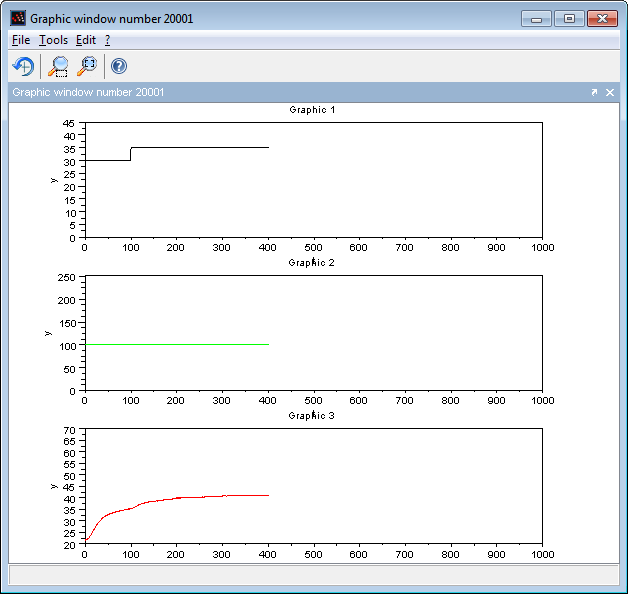
\includegraphics[width=\linewidth]{plot}
\caption{}
\end{figure}
The plot thus obtained is  reasonably good. We obtain $\tau = 68.26, K = 0.700$ and the least square error to be $ 19.92$.\\
The Transfer Function thus obtained is
\begin{align}
G(s)&=\frac{0.700}{68.26s+1}
\end{align}
\newpage
\textbf{Variation}\\
\begin{itemize}
\item It would have been noticed that the experiment is been performed by varying heater current and keeping the fan speed to be constant. However, the user is encouraged to introduce variations in the experiments by choosing different combinations of fan speed and heater current. 
\item Negative ramp can also be introduced to make the experiment more informative. 
\item One can even need not keep a particular input constant. By varying both the inputs, one can imagine it to be like a step varying disturbance signal.
\item The system can also be treated as a second order system. This consideration is however necessary since it increases the accuracy of the acquired transfer function.
\end{itemize}
\newpage
\textbf{Reference:} \\
Modern Control Engineering, 4th Edition, Katsuhiko Ogata, Prentice-Hall India.\\
\newpage
\textbf{Scilab Codes}
\begin{itemize}

\item Scilab code \textquoteleft label.sci\textquoteleft
\vspace{0.5cm}  \\ \textrightarrow function label(tname,tfont,labelx,labely,xyfont)\\
\textrightarrow a = get("current\textunderscore axes")\\
\textrightarrow xtitle(tname,labelx,labely)\\
\textrightarrow xgrid\\
\textrightarrow t = a.title;\\
\textrightarrow t.font\textunderscore size = tfont; //Title font size\\
\textrightarrow t.font\textunderscore style = 2; //Title font style\\
\textrightarrow t.text = tname;\\

\textrightarrow u = a.x\textunderscore label;\\
\textrightarrow u.font\textunderscore size = xyfont; //Label font size\\
\textrightarrow u.font\textunderscore style = 2; //Label font style\\

\textrightarrow v = a.y\textunderscore label;\\
\textrightarrow v.font\textunderscore size = xyfont; //Label font size\\
\textrightarrow v.font\textunderscore style = 2; //Label font style\\

\textrightarrow // a.label\textunderscore font\textunderscore size = 3;\\

\item Scilab code \textquoteleft approx\textunderscore ramp.sci\textquoteright
\vspace{0.5cm}\\ \textrightarrow function lsterr = approx\textunderscore step(T,u,y,input\_slope,tau,limits,no)\\
\textrightarrow t0 = T(1); delta\_u = u(2) - u(1);\\
\textrightarrow u = u - u(1); y = y - y(1);\\
\textrightarrow y\_prediction = gain*input\_slope*((T-t0)-tau+tau*(exp(-(T-t0)/tau)));\\
\textrightarrow format('v',6);\\
\textrightarrow lsterr = norm(y-y\_prediction,2);\\
\textrightarrow ord = [u y y\_prediction]; x = [T T T];\\
\textrightarrow xbasc(); plot2d(x,ord,rect=limits), xgrid();\\
\textrightarrow title = 'Comparison of model with data (tau='\\
\textrightarrow title = title+string(tau)+', K='+string(gain)+',error='+string(lsterr)+')'\\
\textrightarrow label(title,4,'time (s)','Change in temperature (K)',4);\\


\item Scilab code \textquoteleft first.sce\textquoteright.
\vspace{0.5cm}\\ \textrightarrow clear data7; exec('ramp\_final.txt'); \textrightarrow getf('label.sci');\\
\textrightarrow T = data7(:,1); fan = data7(:,3); //T is time, fan is fan speed\\
\textrightarrow u = data7(:,2); y = data7(:,4); // u is current, y is temperature\\
\textrightarrow ord = [u y]; x = [T T]; // u and y are plotted vs. time and time\\
\textrightarrow xbasc(); plot2d(x,ord); xgrid();\\
\textrightarrow title = 'Ramp change in current and the resulting temperature'\\
\textrightarrow label(title,4,'time (s)','Current, Temperature (C)',4);\\
  


\item  Scilab code \textquoteleft approx\textunderscore ramp.sce\textquoteright
\vspace{0.5cm}\\ \textrightarrow clear data7; exec('step1.txt');\\
\textrightarrow getf('label.sci');\\
\textrightarrow getf('approx\textunderscore ramp.sci');\\
\textrightarrow T = data7(:,1); //T is time\\
\textrightarrow u = data7(:,2); y =(data7(:,4) - data7(1,4)); // u is current, y is temperature\\
\textrightarrow N = 200; input\_slope = 0.2;\\
\textrightarrow e = [T y];\\
\textrightarrow f = e(length(u)-N:length(u),:);\\
\textrightarrow g = f(:,1);\\
\textrightarrow h = (g-g)+1;\\
\textrightarrow i = [g h];\\
\textrightarrow j = f(:,2);\\
\textrightarrow l = inv(i'*i)*i'*j\\
\textrightarrow gain = l(1,1)/(input\_slope)\\
\textrightarrow z = -(l(2,1)/(gain*input\_slope))\\
\textrightarrow tau = z; limits = [0,0,250,40]; no=4000;\\
\textrightarrow lsterr = approx\_ramp(T,u,y,input\_slope,tau,limits,no);\\
\end{itemize}
\end{document}
